%%%%%%%%%%%%%%%%%%%%%%%%%%%%%%%%%%%%%%%%%%%%%%%%%%%%%%%%%%%%%%%%%%%%%%%%%%%%%%%
%                                                                             %
% Copyright (C) 2006,2008,2012-2014 Edward d'Auvergne                         %
%                                                                             %
% This file is part of the program relax (http://www.nmr-relax.com).          %
%                                                                             %
% This program is free software: you can redistribute it and/or modify        %
% it under the terms of the GNU General Public License as published by        %
% the Free Software Foundation, either version 3 of the License, or           %
% (at your option) any later version.                                         %
%                                                                             %
% This program is distributed in the hope that it will be useful,             %
% but WITHOUT ANY WARRANTY; without even the implied warranty of              %
% MERCHANTABILITY or FITNESS FOR A PARTICULAR PURPOSE.  See the               %
% GNU General Public License for more details.                                %
%                                                                             %
% You should have received a copy of the GNU General Public License           %
% along with this program.  If not, see <http://www.gnu.org/licenses/>.       %
%                                                                             %
%%%%%%%%%%%%%%%%%%%%%%%%%%%%%%%%%%%%%%%%%%%%%%%%%%%%%%%%%%%%%%%%%%%%%%%%%%%%%%%


% relax development.
%%%%%%%%%%%%%%%%%%%%

\chapter{relax development} \label{ch: relax devel}

This chapter is for developers or those who would like to extend the functionality of relax.
It is not required for using relax.
If you would like to make modifications to the relax source code please subscribe to all the relax mailing lists\index{mailing list} (see the free software infrastructure chapter for more details).
Announcements are sent to ``relax-announce at gna.org''\index{mailing list!relax-announce} whereas ``relax-users at gna.org''\index{mailing list!relax-users} is the list where discussions about the usage of relax should be posted.
``relax-devel at gna.org''\index{mailing list!relax-devel} is where all discussions about the development of relax including feature requests, program design, or any other discussions relating to relax's structure or code should be posted.
Finally, ``relax-commits at gna.org''\index{mailing list!relax-commits} is where all changes to relax's code and documentation, as well as changes to the web pages, are automatically sent to.
Anyone interested in joining the project should subscribe to all four lists.



% Version control using Subversion.
%~~~~~~~~~~~~~~~~~~~~~~~~~~~~~~~~~~

\section{Version control using Subversion}\label{svn repository}

The development of relax requires the use of the Subversion\index{Subversion|textbf} (SVN)\index{SVN|textbf} version control software downloadable from \href{http://subversion.tigris.org/}{http://subversion.tigris.org/}.
The source code to relax is stored in an SVN repository located at \href{http://svn.gna.org/svn/relax/}{http://svn.gna.org/svn/relax/}.
Every single change which has ever made to the program is recorded within this repository\index{repository}.
For more information see the free software infrastructure chapter~\ref{ch: free software} on page~\pageref{ch: free software}.

Although the downloadable distribution archives\index{distribution archive} can be modified it is best that the most current and up to date revision (the \textit{head} revision) is modified instead.
More information about the basics of version control and how this is implemented in Subversion can be found in the Subversion book located at \href{http://svnbook.red-bean.com/}{http://svnbook.red-bean.com/}.

If you are not currently a relax developer you can check out the head revision by typing

\example{\$ svn co svn://svn.gna.org/svn/relax/trunk relax-trunk}

Otherwise if you are a developer type

\example{\$ svn co svn+ssh://xxxxx@svn.gna.org/svn/relax/trunk relax-trunk}

replacing \prompt{xxxxx} with your Gna!\ login name.
If your version is out of date it can be updated to the latest revision by typing

\example{\$ svn up}

Modifications can be made to these sources.



% Coding conventions.
%~~~~~~~~~~~~~~~~~~~~

\section{Coding conventions}

The following conventions should be followed at all times for any code to be accepted into the relax repository.
A Python script which tests if code meets relax's coding conventions is distributed with relax and is located at \file{scripts\ossep{}code\osus{}validator}.
The main reason for these conventions is for readability.
By using a consistent coding style and a high comment ratio, the code becomes much easier to read for non-coders and those new to Python.
It significantly decreases the barrier of entry into the relax source code for NMR spectroscopists.



% Indentation.
\subsection{Indentation}

\index{indentation|textbf}
Indentation should be set to four spaces rather than a tab character.
This is the recommendation given in the Python style guide found at \href{http://www.python.org/doc/essays/styleguide.html}{http://www.python.org/doc/essays/styleguide.html}.
Emacs should automatically set the tabstop correctly.
For vi add the following lines to the \file{vimrc} file:

\begin{exampleenv}
set tabstop=4 \\
set shiftwidth=4 \\
set expandtab
\end{exampleenv}

For UNIX systems, including GNU/Linux and Mac OS X, the \file{vimrc} file is \file{$\sim$\ossep{}.vimrc} whereas in MS Windows the file is \file{\$VIM\ossep{}\_vimrc} which is usually \file{C:$\backslash$Program Files$\backslash$vim$\backslash$\osus{}vimrc}.
Certain versions of vim, those within the 6.2 series, contain a bug where the tabstop value cannot be changed using the \file{vimrc} file (although typing \promptstring{:set tabstop=4} in vim will fix it).
One solution is to edit the file \file{python.vim} which on GNU/Linux systems is located in the path \directory{\ossep{}usr\ossep{}share\ossep{}vim\ossep{}ftplugin\ossep{}}.
It contains the two lines

\begin{exampleenv}
" Python always uses a `tabstop' of 8. \\
setlocal ts=8
\end{exampleenv}

If these lines are deleted the bug will be removed.
Another way to fix the problem is to install newer versions of the run-time files (which will do the same thing).



% Doc strings.
\subsection{Doc strings}
\index{doc string|textbf}

The following are relax's conventions for docstrings.
Many of these are Python conventions.
\begin{itemize}
  \item The standard Python convention of a one line description separated from a detailed description by an empty line should be adhered to.
    This line must start with a capital letter and end in a period.
    This convention is required for certain docstring parsers (see the Python docs).
  \item All functions should have a docstring describing in detail the function, structure, and organisation of the code.
  \item A docstring should be followed by an empty line.
  \item Indentation of the docstring should be the same as that of the first line of code, excluding indented lists, etc.
\end{itemize}

An example of a single line docstring is:

\begin{lstlisting}
    def delete(self):
        """Function for deleting all model-free data."""
\end{lstlisting}

An example of a multiline docstring is:

\begin{lstlisting}
def aic(chi2, k, n):
    """Akaike's Information Criteria (AIC).

    The formula is::

        AIC = chi2 + 2k


    @param chi2:    The minimised chi-squared value.
    @type chi2:     float
    @param k:       The number of parameters in the model.
    @type k:        int
    @param n:       The dimension of the relaxation data set.
    @type n:        int
    @return:        The AIC value.
    @rtype:         float
    """

    return chi2 + 2.0*k
\end{lstlisting}

In addition to the text descriptions, the docstrings use the \href{http://epydoc.sourceforge.net/}{Epydoc}\index{epydoc} markup language to describe arguments, return values, and other information about the code.
See \href{http://epydoc.sourceforge.net/fields.html}{http://epydoc.sourceforge.net/fields.html} for a listing of all the epydoc fields allowed.
This mark up language is important for the creation of the \href{http://www.nmr-relax.com/api/}{API documentation}\index{API documentation} and to help developers understand the purpose and operation of the code.


% Variable, function, and class names.
\subsection{Variable, function, and class names}

In relax a mixture of both camel case (e.g.\ CamelCase)\index{camel case} and lower case with underscores is used.
Despite the variability there are fixed rules which should be adhered to.
These naming conventions should be observed at all times.



% Variables and functions.
\subsubsection{Variables and functions}

For both variables and functions lower case with underscores between words is always used.
This is for readability as the convention is much more fluent than camel case.
A few rare exceptions exist, an example is the Brownian diffusion tensor parameter of anisotropy $\Diff_a$ which is referenced as \prompt{cdp.diff\_tensor.Da}.
As a rule though all new variable or function names should be kept as lower case.
An example of this convention for both the variable name and function name is:

\begin{lstlisting}
    def assemble_param_vector(self, spin=None, spin_id=None, sim_index=None, model_type=None):
        """Assemble the model-free parameter vector (as numpy array).

        If the spin argument is supplied, then the spin_id argument will be ignored.

        @keyword spin:          The spin data container.
        @type spin:             SpinContainer instance
        @keyword spin_id:       The spin identification string.
        @type spin_id:          str
        @keyword sim_index:     The optional MC simulation index.
        @type sim_index:        int
        @keyword model_type:    The optional parameter set, one of 'all', 'diff', 'mf', or 'local_tm'. 
        @type model_type:       str or None
        @return:                An array of the parameter values of the model-free model.
        @rtype:                 numpy array
        """

        # Initialise.
        param_vector = []

        # Determine the model type.
        if not model_type:
            model_type = self.determine_param_set_type()

        # Diffusion tensor parameters.
        if model_type == 'diff' or model_type == 'all':
            # Normal parameters.
            if sim_index == None:
                # Spherical diffusion.
                if cdp.diff_tensor.type == 'sphere':
                    param_vector.append(cdp.diff_tensor.tm)
\end{lstlisting}



% Classes.
\subsubsection{Classes}

For classes relax uses a mix of camel case (for example all the \prompt{RelaxError} objects) and underscores (for example \pycode{Model\_free}).
The first letter in all cases is always capitalised.
Generally the camel case is reserved for very low level classes which are involved in the program's infrastructure.
Examples include the RelaxError code, the threading code, and the relax data store code.
All the data analysis specific code, generic code, interface code, etc.\ uses underscores between the words with only the first letter capitalised.
One exception is the space mapping class \pycode{OpenDX}, the reason being that the program is called \prompt{OpenDX}.
An example is:

\begin{lstlisting}
class Model_free_main:
    """Class containing functions specific to model-free analysis."""

    def are_mf_params_set(self, spin):
        """Test if the model-free parameter values are set.

        @param spin:    The spin container object.
        @type spin:     SpinContainer instance
        @return:        The name of the first parameter in the parameter list in which the corresponding parameter value is None.  If all parameters are set, then None is returned.
        @rtype:         str or None
        """

        # Deselected residue.
        if spin.select == 0:
            return
\end{lstlisting}



% Long names.
\subsubsection{Long names}

If you have a look at a few relax source files, you will notice that the variable, function, and class names can be quite long.
For example the model-free function \pycode{disassemble\_param\_vector()} and the RelaxError class \pycode{RelaxNoSequenceError}.
While this is not normal for coding, it is an important component of relax as it facilitates the reading of the source code by a non-coder or someone not familiar with the codebase.
Iteration counters can be single letter variables such as \pycode{i}, \pycode{j}, \pycode{k}, etc., however for all other variables, functions, and classes please attempt to use descriptive names which are instantly identifiable.
Please minimise the amount of abbreviations used and only use those which are obvious.
For example naming the parameter vector \pycode{self.param\_vector}, the relaxation data \pycode{relax\_data}, the model selection class \pycode{class Model\_selection}, the type of spheroidal diffusion \pycode{spheroid\_type}, etc.



% Whitespace.
\subsection{Whitespace}

The following conventions are for general code cleanliness and readability:
\begin{itemize}
  \item Trailing whitespace should be avoided, although this is not very important.
  \item All functions should be preceded by two empty lines.
    The only exception is the first function of the class definition.
  \item Function arguments should be separated by a comma followed by a single space.
  \item The assignment operator should be surrounded by spaces, for example \verb*!tm = 1e-8!.
    The exception is function arguments where for example \verb*!self.classic\_colour(res\_num=None, width=0.3)!.
  \item The comparison operators should also be surrounded by spaces, e.g.\ \verb*! < !, \verb*! > !, \verb*! == !, \verb*! <= !, \verb*! => !, \verb*! <> !, \verb*! != !, \verb*! is !, and \verb*! in !.
\end{itemize}

An example which shows most of these conventions is:
\begin{lstlisting}
class Internal:
    """The internal relax structural data object.

    The structural data object for this class is a container possessing a number of different arrays corresponding to different structural information.  These objects are described in the structural container docstring.
    """

    def _bonded_atom(self, attached_atom, index, mol):
        """Find the atom named attached_atom directly bonded to the atom located at the index.

        @param attached_atom:   The name of the attached atom to return.
        @type attached_atom:    str
        @param index:           The index of the atom which the attached atom is attached to.
        @type index:            int
        @param mol:             The molecule container.
        @type mol:              MolContainer instance
        @return:                A tuple of information about the bonded atom.
        @rtype:                 tuple consisting of the atom number (int), atom name (str), element name (str), and atomic position (Numeric array of len 3)
        """

        # Init.
        bonded_found = False

        # No bonded atoms, so determine the connectivities.
        if not mol.bonded[index]:
            # Determine the molecule type if needed.
            if not hasattr(mol, 'type'):
                self._mol_type(mol)
\end{lstlisting}



% Comments.
\subsection{Comments}

Comments are a very important component within relax.
In the current source code the percentage of comment lines relative to lines of code ranges from 15\% to over 30\% for different files.
The average comment density would be close to 25\%.
The purpose of having so many comment lines, much more than you would expect from source code, is so that the relax's code is fully self documented.
It allows someone who is not familiar with the codebase to read the code and quickly understand what is happening.
It simplifies the process of learning and allows NMR spectroscopists who are not coders to dive into the code.
If writing code for relax, please attempt to maintain the tradition by aiming towards a 25\% comment ratio.
The comment should be descriptive of what the code below it is supposed to do.
Most importantly the comment explains why that code exists.
The script \file{scripts\ossep{}code\osus{}validator} can be used to check the comment density.



% Submitting changes to the relax project.
%~~~~~~~~~~~~~~~~~~~~~~~~~~~~~~~~~~~~~~~~~

\section{Submitting changes to the relax project}


% Submitting changes as a patch.
\subsection{Submitting changes as a patch}
\index{patch|textbf}

The preferred method for submitting fixes and improvements to the relax source code is by the creation of a patch.
If your changes are a fix make sure you have submitted a bug report\index{bug!report} to the bug tracker\index{bug!tracker} located at \href{https://web.archive.org/web/https://gna.org/bugs/?group=relax}{https://web.archive.org/web/https://gna.org/bugs/?group=relax} first.
See section~\ref{reporting bugs} on page~\pageref{reporting bugs} for more details.
Two methods can be used to generate the patch -- the Unix command \file{diff} or the Subversion program.
The resultant file \file{patch} of either the \file{diff} or \file{svn} command described below can be posted to the ``relax-devel at gna.org'' mailing list\index{mailing list!relax-devel}.
Please label within your post which version of relax you modified or which revision the patch is for.
Also try to create a commit log\index{commit log} message according to the format described in section~\ref{commit log format} on page~\pageref{commit log format} for one of the relax committers to use as a template for committing the change.



% Modification of official releases -- creating patches with diff.
\subsection{Modification of official releases -- creating patches with diff}
\index{patch!diff|textbf}

If your modifications have been made to the source code of one of the official relax releases (for example 2.1.1) then the Unix command \file{diff} can be used to create a patch.
A patch file is simply the output of the diff command run with the recursive flag and presented in the `unified' format.
Therefore two directories need to be compared.
If the original sources are located in the directory \directory{relax\osus{}orig} and the modified sources in \directory{relax\osus{}mod} then the patch can be created by typing

\example{\$ diff -ur relax\_orig relax\_mod > patch}



% Modification of the latest sources -- creating patches with Subversion.
\subsection{Modification of the latest sources -- creating patches with Subversion}
\index{patch!Subversion|textbf}
\index{Subversion!patch|textbf}

If possible changes to the latest sources is preferred.
Using the most up to date sources from the relax SVN repository will significantly aid the relax developers to incorporate your changes back into the main development line.
To check out the current development line see section~\ref{svn repository} on page~\pageref{svn repository} for details.
Prior to submitting a patch to the mailing list your sources should be updated to include the most recent changes.
To do this type

\example{\$ svn up}

and note the revision number to include in your post.
The update may cause a conflict if changes added to the repository clash with your modifications.
If this occurs see the Subversion book at \href{http://svnbook.red-bean.com/}{http://svnbook.red-bean.com/} for details on how to resolve the conflict or submit a message to the rela\mbox{x-d}evel list\index{mailing list!relax-devel}.

Once the sources are up to date your changes can be can be converted into the patch text file.
Using SVN creating a patch is easy.
Just type

\example{\$ svn diff > patch}

in the base relax directory.



% Committers.
%~~~~~~~~~~~~

\section{Committers}


% Becoming a committer.
\subsection{Becoming a committer}\label{becoming a committer}

Anyone can become a relax developer and obtain commit access\index{commit access} to the relax repository.
The main criteria for selection by the relax developers is to show good judgement, competence in producing good patches, compliance with the coding and commit log conventions, comportment on the mailing lists, not producing too many bugs, only taking on challenges which can be handled, and the skill in judging your own abilities.
You will also need to have an understanding of the concepts of version control specifically those relating to Subversion\index{Subversion}.
The SVN book at \href{http://svnbook.red-bean.com/}{http://svnbook.red-bean.com/} contains all the version control information you will need.
After a number of patches have been submitted and accepted any of the relax developers can propose that you receive commit access.
If a number of developers agree while no one says no then commit access will be offered.

One area where coding ability can be demonstrated is within the relax test suite\index{test suite}.
The addition of tests, especially those where the relax internal data structures of the relax data store are scrutinised, can be a good starting point for learning the structure of relax.
This is because the introduction of bugs has no effect on normal program execution.
The relax test suite is an ideal proving ground.

If skills in only certain areas of relax development, for example in creation of the documentation, an understanding of C but not python, an understanding of solely the code of the user interface, or an understanding of the code specific to a certain type of data analysis methodology, then partial commit access may be granted.
Although you will have the ability to make modifications to any part of the repository please make modifications only those areas for which you have permission.



% Joining Gna!
\subsection{Joining Gna!}
\index{Gna}

The first step in becoming a committer is to create a Gna!\ account.
Go to \href{https://web.archive.org/web/https://gna.org/account/register.php}{https://web.archive.org/web/https://gna.org/account/register.php} and type in a login name, password, real name, and the email address you would like to use.
You will then get an automatic email from Gna!\ which will contain a link to activate your registration.



% Joining the relax project.
\subsection{Joining the relax project}

The second step in becoming a committer is to register to become a member of the relax project.
Go to the Gna!\ website\index{Gna} (\href{https://web.archive.org/web/https://gna.org/}{https://web.archive.org/web/https://gna.org/}) and login.
Click on `My Groups' to go to \href{https://web.archive.org/web/https://gna.org/my/groups.php}{https://web.archive.org/web/https://gna.org/my/groups.php}.
In the section `Request for inclusion' type `relax' and hit enter.
Select relax and write something in the comments.
If you have been approved (see section~\ref{becoming a committer}) you will be added to the project committers list.



% Format of the commit logs.
\subsection{Format of the commit logs}\label{commit log format}
\index{commit log|textbf}

If you are a relax developer and you have commit access to the repository the following conventions should be followed for all commit messages.
\begin{itemize}
  \item The length of all lines in the commit log should never exceed 100 characters.
    This is so that the log message viewed in either emails or by the command prompt command \mbox{\prompt{svn log}} is legible.
  \item The first line of the commit log should be a short description or synopsis of the changes.
    If the change relates to a bug or a task, include the bug and task number using the notation \texttt{type \#num} where type is either \texttt{bug}, \texttt{task} or \texttt{support} and \texttt{num} is the id number (for example \texttt{bug \#6503}).
    This terminology is important because the Gna!\ infrastructure knows how to translate this into a link to the issue.
    Also include a link to the issue.
  \item The second line should be blank.
  \item If the commit is a bug fix reported by a non-committer or if the commit originates from a patch posted by a non-committer the next lines should be reserved for crediting.
    The name of the person and their obfuscated email address (for example edward \_at\_ nmr-relax \_dot\_ com) should be included in the message.
  \item Next should be another blank line.
  \item If the commit relates to an entry in the bug tracker or to a discussion on the mailing lists then the web address of either the bug report or the mailing list archive message should be cited in the next section (separated from the synopsis or credit section by a blank line).
    All relevant links should be included to allow easy navigation between the repository\index{repository}, mailing lists\index{mailing list}, bug tracker\index{bug!tracker}, etc.
    An example is bug \#5559 which is located at \href{https://web.archive.org/web/https://gna.org/bugs/?func=detailitem\&item\_id=5559}{https://web.archive.org/web/https://gna.org/bugs/?func=detailitem\&item\_id=5559} and the post to ``relax-devel at gna.org''\index{mailing list!relax-devel} describing the fix to that bug which is located at \href{https://web.archive.org/web/https://mail.gna.org/public/relax-devel/2006-03/msg00013.html}{https://web.archive.org/web/https://mail.gna.org/public/relax-devel/2006-03/msg00013.html}.
  \item A full description with all the details can follow.
    This description should follow a blank line, can itself be sectioned using blank lines, and finally the log is terminated by one blank line at the end of the message.
\end{itemize}

An example of a commit message for the closure of a bug is:

\begin{exampleenv}
Fixing the rest of bug \#7241 (\href{https://web.archive.org/web/https://gna.org/bugs/?7241}{https://web.archive.org/web/https://gna.org/bugs/?7241}).

Bug \#7241 was thought to be fixed in in r2591 and r2593, the commit messages describing the solution
being located at \href{https://web.archive.org/web/https://mail.gna.org/public/relax-commits/2006-09/msg00064.html}{https://web.archive.org/web/https://mail.gna.org/public/relax-commits/2006-09/msg00064.html} (Message-id:
<E1GTgBi-0000R6-4h@subversion.gna.org>) for r2591 and
\href{https://web.archive.org/web/https://mail.gna.org/public/relax-commits/2006-10/msg00001.html}{https://web.archive.org/web/https://mail.gna.org/public/relax-commits/2006-10/msg00001.html} (Message-id:
<E1GTt6C-0005rk-8q@subversion.gna.org>) for r2593.

However this was not the only place that the Scientific Python PDB data structure peptide\_chains was
being accessed.  The chains were being accessed in the file `pipe\_control/sequence.py' when the
sequence was being read out of the PDB file.  This has now been modified with changes similar to
r2591 and r2593.
\end{exampleenv}

An example of a commit message for changes relating to a task is:

\begin{exampleenv}
This change implements half of task \#3630 (\href{https://web.archive.org/web/https://gna.org/task/?3630}{https://web.archive.org/web/https://gna.org/task/?3630}).

The docstring in the generic optimisation function has been modified to clear up the ambiguity cased
by supplying the option `None' together with Newton optimisation.
\end{exampleenv}

One last commit message example is:

\begin{exampleenv}
Added the API documentation creation (using Epydoc) to the Scons scripts.

The Scons target to create the HTML API documentation is called `api\_manual\_html'.  The
documentation can be created by typing:
\$ scons api\_manual\_html

The function `compile\_api\_manual\_html()' was added to the `scons/manuals.py' file.  This function
runs the `epydoc' command.  All the Epydoc options are specified in that function.
\end{exampleenv}



% Discussing major changes.
\subsection{Discussing major changes}

If you are contemplating major changes, either for a bug fix, to add a completely new feature or user function for your own work, to improve the behaviour of part the program, or any other potentially disruptive modifications, please discuss these ideas on the rela\mbox{x-d}evel mailing list\index{mailing list!relax-devel}.
If the planned changes have the potential to introduce problems the creation of a private branch may be suggested.



% Branches.
\section{Branches}
\index{branches|textbf}
\index{repository!branches|textbf}


\subsection{Branch creation}
\index{repository!branch creation}

If a change is likely to be disruptive or cause breakages in the program, the use of your own temporary branch is recommended.
This private branch is a complete copy of one of the main development lines wherein you can make changes without disrupting the other developers.
Although called a private branch every change is visible to all other developers and each commit will result in an automatic email to the relax-commits mailing list\index{mailing list!relax-commits}.
Other developers are even able to check out your branch and make modifications to it.
Private branches can also be used for testing ideas.
If the idea does not work the branch can be deleted from the repository (in reality the branch will always exist between the revision numbers of its creation and deletion and can always be resurrected).
For example to create a branch from the main development line, the `trunk', called \prompt{molmol\_macros} whereby new Molmol macros are to be written, type

\begin{exampleenv}
\$ svn cp svn+ssh://xxxxx@svn.gna.org/svn/relax/trunk $\backslash$ \\
 svn+ssh://xxxxx@svn.gna.org/svn/relax/branches/molmol\_macros
\end{exampleenv}

replacing \prompt{xxxxx} with your login name.
You can then check out your private branch by typing

\example{\$ svn co svn+ssh://xxxxx@svn.gna.org/svn/relax/branches/molmol\_macros}

which will create a directory called \directory{molmol\osus{}macros} containing all the relax source files.
To have the files placed into a different directory, type the name of that directory at the end of the last command.
Modifications can be made to this copy while normal development continues on the main line.


\subsection{Keeping the branch up to date using \file{svnmerge.py}}
\index{svnmerge.py}
\index{repository!keeping up to date}
\index{repository!svnmerge.py}

As you develop your branch, changes will be occurring simultaneously within the main line.
These changes should be merged into your branch on a regular basis to avoid large incompatible changes from forming between the two branches.
To simplify this process, the \file{svnmerge.py} script located at \href{http://www.orcaware.com/svn/wiki/Svnmerge.py}{http://www.orcaware.com/svn/wiki/Svnmerge.py} can be used.
It is best to download the trunk version from that page, unless that version is non-functional.
Once you have this script, the merging from the main line to your private branch must be initialised by typing, from within the checked out copy of your branch,

\example{\$ svnmerge.py init}
\index{Subversion!svnmerge.py init}

This then needs to be committed using the automatically generated log

\example{\$ svn ci -F svnmerge-commit-message.txt}
\index{Subversion!commit}

To keep up to date, simply type

\example{\$ svnmerge.py merge}
\index{Subversion!svnmerge.py merge}


If conflicts\index{Subversion!conflict} have occurred please refer to the Subversion book at \href{http://svnbook.red-bean.com/}{http://svnbook.red-bean.com/} for information on how to resolve the problem.
Otherwise, or once fixed, the main line revisions merged into your branch can be committed using the automatically generated log file:

\example{\$ svn ci -F svnmerge-commit-message.txt}
\index{Subversion!commit}


\subsection{Merging the branch back into the main line}
\index{repository!merging branch back}

Once you have completed the modifications desired for your branch, all changes which have occurred in the main line have been merged using \file{svnmerge.py}, and the changes have been approved for merging back into the main line -- then your branch can be merged.
First check out a copy of the main line,

\example{\$ svn co svn+ssh://xxxxx@svn.gna.org/svn/relax/trunk relax-trunk}
\index{Subversion!check out}

or update a previously checked out version,

\example{\$ svn up}
\index{Subversion!update}

Then \file{svnmerge.py} can be utilised again.
First initialise the merging process by typing, from within the checked out copy of the main line, 

\example{\$ svnmerge.py init svn+ssh://xxxxx@svn.gna.org/svn/relax/branches/molmol\_macros}
\index{Subversion!svnmerge.py init}

Then commit the change

\example{\$ svn ci -F svnmerge-commit-message.txt}
\index{Subversion!commit}

To merge the branch and commit the changes, type

\example{\$ svnmerge.py merge --bidirectional}
\index{Subversion!svnmerge.py merge}

\example{\$ svn ci -F svnmerge-commit-message.txt}
\index{Subversion!commit}

Finally the merge properties need to be removed

\example{\$ svnmerge.py uninit -S svn+ssh://xxxxx@svn.gna.org/svn/relax/branches/molmol\_macros}
\index{Subversion!svnmerge.py uninit}
\index{Subversion!merge}

the changes committed

\example{\$ svn ci -F svnmerge-commit-message.txt}
\index{Subversion!commit}

and your private branch deleted

\example{\$ svn rm svn+ssh://xxxxx@svn.gna.org/svn/relax/branches/molmol\_macros}
\index{Subversion!remove}



% The SCons build system.
%~~~~~~~~~~~~~~~~~~~~~~~~

\section{The SCons build system}
\index{SCons|textbf}

The \href{http://www.scons.org/}{SCons} build system was chosen over other build systems including \prompt{make}\index{make} as it is a cross-platform build system which can be used in Unix\index{Operating system!Unix}, GNU/Linux\index{Operating system!GNU/Linux}, Mac OS X\index{Operating system!Mac OS X}, and even MS Windows\index{Operating system!MS Windows} (the correct compilers are nevertheless required).
Various components of the program relax can be created using the SCons utility.
This includes C module compilation, manual creation, distribution creation, and cleaning up and removing certain files.
The file \file{sconstruct} in the base relax directory, which consists of python code, directs the operation of SCons for the various functions.



% SCons help.
\subsection{SCons help}
\index{SCons!help|textbf}

Multiple functions have been built into the \file{sconstruct} script and the modules of the \directory{scons} directory.
Each of these can be selected by specifying different ``targets'' when running SCons.
A description of each target is given by the SCons help system which is accessible by typing \prompt{scons --help} in the base relax directory.



% C module compilation.
\subsection{C module compilation}
\index{C module compilation|textbf}
\index{SCons!C module compilation|textbf}

As described in the installation chapter, typing \prompt{scons} in the base directory will create the shared objects or dll files which are imported into Python as modules.



% Compilation of the PDF manual.
\subsection{Compilation of the user manual (PDF version)}
\index{user manual!PDF compilation|textbf}

To create the PDF version of the relax user manual type

\example{\$ scons user\_manual\_pdf}
\index{SCons!user manual (PDF version)|textbf}

in the base directory.
SCons will then run a series of shell commands to create the manual from the \LaTeX\ sources located in the \directory{docs\ossep{}latex} directory.
This is dependent on the programs \file{latex}, \file{makeindex}, \file{dvips}, and \file{ps2pdf} being located within the environment's path.



% Compilation of the HTML manual.
\subsection{Compilation of the user manual (HTML version)}
\index{user manual!HTML compilation|textbf}

The HTML version of the relax user manual is made by typing

\example{\$ scons user\_manual\_html}
\index{SCons!user manual (HTML version)|textbf}

in the base directory.
One command calling the program \file{latex2html} will be executed which will create HTML pages from the \LaTeX\ sources.



% Compilation of the API documentation.
\subsection{Compilation of the API documentation (HTML version)}
\index{API documentation|textbf}

The HTML version of the relax API documentation is made by typing

\example{\$ scons api\_manual\_html}
\index{SCons!API documentation|textbf}

in the base directory.
The programs Epydoc and Graphviz are required for creating this documentation.
The resultant HTML pages will be located in the directory \directory{docs\ossep{}api}.



% Making distribution archives.
\subsection{Making distribution archives}
\index{distribution archive|textbf}

Two types of distribution archive can be created from the currently checked out sources -- the source and binary distributions.
To create the source distribution type 

\example{\$ scons source\_dist}
\index{SCons!source distribution|textbf}

whereas to create the binary distribution, whereby the C modules are compiled and the resultant shared objects are included in the bzipped tar file, type

\example{\$ scons binary\_dist}
\index{SCons!binary distribution|textbf}

If a binary distribution does not exist for your architecture feel free to create it yourself and contribute the archive to be included on the download pages.
To do this you will need to check out the appropriate tagged branch from the relax subversion repository.
If the current stable release is called 1.2.3 check out that branch by typing

\example{\$ svn co svn+ssh://bugman@svn.gna.org/svn/relax/tags/1.2.3 relax}
\index{Subversion!check out}

replacing \prompt{bugman} with your user name if you are a relax developer, otherwise typing

\example{\$ svn co svn://svn.gna.org/svn/relax/tags/1.2.3 relax}
\index{Subversion!check out}

Then build the binary distribution and send a message to the relax development mailing list\index{mailing list!relax-devel}.
If compilation does not work please submit a bug to the bug tracker\index{bug!tracker} system at \href{https://web.archive.org/web/https://gna.org/bugs/?group=relax}{https://web.archive.org/web/https://gna.org/bugs/?group=relax} detailing the relax version, operation system, architecture, and any other information you believe will help to solve the problem.
More information about donating binary distributions to the relax project is given in the free software infrastructure chapter (Chapter~\ref{ch: free software}, page~\pageref{ch: free software}).



% Cleaning up.
\subsection{Cleaning up}
\index{clean up|textbf}

If the command

\example{\$ scons clean}
\index{SCons!clean up|textbf}

is run in the base directory all Python byte compiled files \file{*.pyc}, all C object files \file{*.o} and \file{*.os}, and any backup files with the extension \file{*.bak} are removed from all sub-directories.
In addition any temporary \LaTeX\ compilation files are removed from the \directory{docs\ossep{}latex} directory.

The more powerful command

\example{\$ scons clean\_all}

will, in addition to all the files removed by the \prompt{clean} target, remove all compiled C shared object files (\file{*.so}, \file{*.dylib}, \file{*.pyd}) and the \prompt{build} and \prompt{dist} directories created when building the Mac OS X application.



% The core design of relax.
%~~~~~~~~~~~~~~~~~~~~~~~~~~

\section{The core design of relax}

To enable flexibility the internal structure of relax is modular.
By construction the large collection of independent data analysis tools can be used individually and relatively easily by any new code implementing other forms of relaxation data analysis or even by other programs.
The core modular design of the program is shown in Figure~\ref{fig: core design}.



% The divisions of relax's source code.
\subsection{The divisions of relax's source code}

relax's source code can be divided into five major areas:  the initialisation code, the user interface (UI) code, the functional code, the number crunching code, and the code storing the program state.
\begin{description}
  \item[Initialisation:]  The code belonging to this section initialises the program, processes the command-line arguments, and determines what mode the program will be run in including the choice of the UI.
  \item[UI:]  The current UI modes in relax include the prompt, the script and the GUI modes.
    These consist of separate code paths, all sitting on top of the underlying functional code.
    In the future, a web-based interface may be added.
  \item[Functional code:]  This code is the main part of the program.
    It includes anything which does not fit into the other sections and comprises the generic code, the specific code, and the specific setup code used as an interface between the two.
  \item[Number crunching:]  The computationally expensive code belongs in this section.
  \item[Program state:]  The state of the program is contained within the relax data store which is accessible from all parts of the program as a singleton object.
\end{description}

% Core relax design figure.
\begin{figure}
  \centerline{
    \includegraphics[
      width=\textwidth,
      bb=0 -1 389 476
    ]
    {images/core_design}
  }
  \caption{The core design of relax.}
  \label{fig: core design}
\end{figure}



% The major components of relax.
\subsection{The major components of relax}

Each of the boxes in Figure~\ref{fig: core design} represents a different grouping of code.
\begin{description}
  \item[relax:]  The top level module.
    This initialises the entire program, tests the dependencies, sets up the multi-processor framework and specific processor fabric, and prints the program's introduction message.
  \item[Command line arguments:]  This code processes the arguments supplied to the program and decides whether to print the help message, initialise the prompt, execute a script, initialise a different UI, run the program in test mode, or run the program as a slave thread.
  \item[Prompt:]  The main user interface consisting of a Python\index{Python} prompt\index{User interface!prompt|textbf}.
    The namespace of the interpreter contains the various user functions which are front ends to the generic code.
    The user functions are simply Python functions which test the supplied arguments to make sure they are of the correct type (string\index{string}, integer\index{integer}, list\index{list}, or any other type) before sending the values to the generic code.
    The code for the prompt is located in the directory \directory{prompt\ossep{}}.
  \item[Script:]  If a script\index{User interface!scripting|textbf} is supplied on the command line or executed within another user interface it will be run in the same namespace as that of the prompt.
    Hence the script has access to all the user functions available at the relax prompt.
    This allows commands which are typed at the prompt to be pasted directly and unmodified into a text file to be run as a script.
  \item[GUI:]  The graphical user interface\index{User interface!GUI|textbf} code base is located in the \directory{gui} directory.
  \item[Other interfaces:]  Any number of interfaces (for example a web-based interface or an ncurses interface) could be added to relax without modification of the current sources.
    This must be, without question, developed within the relax source code repository otherwise the code will not be maintainable in the future and will be almost impossible back into relax later on.
  \item[Generic code:]  This code includes classes and functions which are independent of the UI and not specific to a certain data pipe type, for example not being involved in model-free analysis, relaxation curve-fitting, the NOE calculation, and reduced spectral density mapping.
    All this code is located in the directory \directory{pipe\osus{}control\ossep{}}.
  \item[Specific setup:]  This code implements the internal interface between the generic and specific code.
    The generic code calls the specific setup asking for a specific function for the given data pipe type.
    For example by asking for the minimise function when the data pipe type is model-free analysis the model-free specific \pycode{minimise()} method is returned.
    Although the generic code accesses the specific code solely through this interface the specific code can access the generic code directly.
    The code is located in the file \file{specific\osus{}fns\ossep{}specific\osus{}setup.py}.
  \item[Specific code:]  This is the code which is specific to the data pipe type -- model-free analysis, relaxation curve-fitting, reduced spectral density mapping, and the NOE calculation.
    Each type is located in a separate file in the directory \directory{specific\osus{}fns\ossep{}}.
  \item[Mathematical functions:]  This is reserved for CPU intensive code involved in calculations.
    The code may be written in Python however C code can be used to significantly increase the speed of the calculations.
    For optimisation the code can include function evaluations, calculation of gradients, and calculation of Hessians.
    These functions are located in the directory \directory{maths\osus{}fns\ossep{}}.
  \item[Data:]  The program state stored in the relax data store singleton object.
    This class contains all the program data and is accessed by the generic and specific code.
    The mathematical functions may also access this data but this is not recommended.  The structure is initialised by the file \file{data\ossep{}\_\_init\_\_.py}.
\end{description}




% The mailing lists.
%~~~~~~~~~~~~~~~~~~~

\section{The mailing lists for development}
\index{mailing list|textbf}


% Private vs. public messages.
\subsection{Private vs.\ public messages}

If you would like to start a private discussion, please label your email as such.
Private messages are however strongly discouraged, only start a private conversation if you really must.

If you receive a reply to a message you have sent, a bug report you have filed, etc.\ which has not been sent to the mailing list and has not been labelled as private, then the most likely explanation is that ``reply-to-all'' has not been used and hence the mailing list has not been included on the CC list.
If this occurs, please ask the person if the message was meant to be private and refrain from discussing any of the comments within the post.
Save these comments until after the person responds by saying that the message was private or re-sends the message to the mailing list.
Try to encourage public messages if you think that the post need not be private and if you think that it would be useful for the mailing list archives.

For thread consistency, if you send a message which accidentally misses the mailing list, please do not then forward the previously sent message to the list.
For better readability of the mailing list archives, it is best that you create an entirely new message responding to the original post.
Just cut and paste your miss-directed message into your new message.
That way the thread will be continuous -- there will not be any messages missing from the middle of the thread in between the original post and your forwarded message.

To simplify the process of checking if the message was supposed to be private, you could copy-and-paste the following message (modifying it as you see fit):

\begin{exampleenv}
Sorry in advance, but the following is the standard pre-composed response to a post not sent to the relax mailing lists and not labelled as private.  If you would like to start a private conversation about relax, please label your message as such.  If you really must start a private exchange, please respond to this message saying so.  If your message was meant to be sent to the relax mailing list, please send the message again.  For this, please copy-and-paste your message, replying to the original (i.e.\ no forwarding), and making sure that the mailing list is in the CC field by clicking on ``reply-to-all''.
\end{exampleenv}




% The bug, task, and support request trackers.
%~~~~~~~~~~~~~~~~~~~~~~~~~~~~~~~~~~~~~~~~~~~~~

\section{The bug, task, and support request trackers}
\index{bug!tracker|textbf}
\index{task!tracker|textbf}
\index{support request!tracker|textbf}
\index{tracker!bug|textbf}
\index{tracker!task|textbf}
\index{tracker!support request|textbf}

relax's infrastructure includes three different issue trackers.
These are the \href{https://web.archive.org/web/https://gna.org/bugs/?group=relax}{bug tracker}, the \href{https://web.archive.org/web/https://gna.org/task/?group=relax}{task tracker}, and the \href{https://web.archive.org/web/https://gna.org/support/?group=relax}{support request tracker}.



% Submitting a bug report.
\subsection{Submitting a bug report}

If someone reports a bug to one of the relax mailing lists, ask that person if they would like to create a bug report for that problem, pointing them to the submission web page.
This is a good starting point to allow the person to become more involved in the relax project.
If they do not respond or say that they would prefer not to, then you can create bug report for the issue linking to the original message and crediting the person for reporting the issue.



% Assigning an issue to yourself.
\subsection{Assigning an issue to yourself}

If you are a relax committer and see an issue which you would like to solve, please assign that issue to yourself before you start work on it.
The assignment will prevent duplicated efforts.
If you can see an area where relax needs work, feel free to create a report within task tracker and then assign the task to yourself.



% Closing an issue.
\subsection{Closing an issue}

When closing an issue (whether a bug report, a task, or a support request) a number of steps need to be taken.
The tracker status should be changed to ``Done'' and the issue ``Closed''.
In addition, a message should be included which states the repository revision and the relax-commits mailing list archive link (with the message-id) in which the issue was solved.
If multiple commits were required, then include all the revisions and as many links as possible (if a task required many commits, the relax-commits links could be skipped).
An example is \href{https://web.archive.org/web/https://gna.org/bugs/?7402}{bug \#7402} where the closing comment was:

\begin{exampleenv}
This documentation bug was fixed in r2641. The commit message is located at \href{https://web.archive.org/web/https://mail.gna.org/public/relax-commits/2006-10/msg00073.html}{https://web.archive.org/web/https://mail.gna.org/public/relax-commits/2006-10/msg00073.html} (Message-id: <E1GYG4l-0002kK-Jx@subversion.gna.org>).
\end{exampleenv}



% Links, links, and more links.
%~~~~~~~~~~~~~~~~~~~~~~~~~~~~~~

\section{Links, links, and more links}
\index{linking|textbf}

Creating links throughout the relax infrastructure is important for two major reasons -- navigation and search engine indexing.
When including a link to a post within the mailing list archives, please include the message-id email header.
This enables subscribers to the mailing lists to search for the specific message within their local copy of the email messages.



% Navigation.
\subsection{Navigation}

To be able to easily navigate between the relax infrastructure components -- the bug tracker, the task tracker, the support request tracker, the relax-devel mailing list, the commit logs, and the SVN and CVS repositories -- try to include as many links as possible.

For example a bug may first be reported on the relax-users mailing list, then placed within the bug tracker, discussed on relax-devel, a fix committed to the repository, and finally the bug report closed.
To be able to follow this chain, links are very important (email message-ids are also important).
When the bug is first added to the bug tracker, a link to the relax-users mailing list archive message and the message-id should be included.
If you start a discussion on relax-devel, try to include links to the bug tracker entry and the relax-users message.
When committing a fix to the repository, include links to the bug report, to the start of the thread in the mailing list archive, and the original message to relax-users.
Then when the bug report is closed, include the revision number of the fix and a link to the relax-commits archive message (and message-id).
By having all these links, it is then very easy for someone else to jump between the systems and follow the progression of the bug fix.

If you send a message referring to an old post which was sent the relax mailing lists, an old bug report, or any other archived information, please take the time to find that original information in the archives and include a link to it (including the message-id if relevant).
It is much more efficient for a single person to hunt down that message than for the many recipients of your post to search for the message themselves.
By including the link, you decrease the overhead of following the mailing list.



% Search engine indexing.
\subsection{Search engine indexing}

Having a large web of links across relax's infrastructure aids in the search engine indexing of the mailing list archives and the \href{http://www.nmr-relax.com}{http://www.nmr-relax.com} web site.
The web of links is useful for catching those Google bots.
That way the Google searching of the mailing list archives located on the \href{http://www.nmr-relax.com/communication.html}{communication web page} will be more up to date.
However to increase the search engine ranking of the web site, links to \href{http://www.nmr-relax.com}{http://www.nmr-relax.com} from external sites is required.
This is one reason why relax can be found at a number of sites across the web:
\begin{description}
  \item[Freecode:]  New relax releases are announced not only on the \href{https://web.archive.org/web/https://mail.gna.org/public/relax-announce/}{relax-announce} mailing list and on the relax \href{https://web.archive.org/web/https://gna.org/news/?group=relax}{news} pages, but also on \href{http://freecode.com/projects/nmr-relax}{Freecode}.
    This used to be called Freshmeat.
  \item[The mail archive:]  This site archives all of the relax mailing lists, including \href{http://mail-archive.com/relax-announce@gna.org/}{relax-announce}, \href{http://mail-archive.com/relax-users@gna.org/}{relax-users}, \href{http://mail-archive.com/relax-devel@gna.org/}{relax-devel}, and \href{http://mail-archive.com/relax-commits@gna.org/}{relax-commits}.
  \item[Gmane:]  Pronounced as ``main'', the relax mailing lists are also archived at Gmane in numerous formats.
    The archived relax mailing lists include relax-announce (\href{http://news.gmane.org/gmane.science.nmr.relax.announce}{thread}, \href{http://blog.gmane.org/gmane.science.nmr.relax.announce}{blog}, \href{nntp://news.gmane.org/gmane.science.nmr.relax.announce}{NNTP}, \href{http://rss.gmane.org/messages/excerpts/gmane.science.nmr.relax.announce}{RSS}), relax-users (\href{http://news.gmane.org/gmane.science.nmr.relax.user}{thread}, \href{http://blog.gmane.org/gmane.science.nmr.relax.user}{blog}, \href{nntp://news.gmane.org/gmane.science.nmr.relax.user}{NNTP}, \href{http://rss.gmane.org/messages/excerpts/gmane.science.nmr.relax.user}{RSS}), relax-devel (\href{http://news.gmane.org/gmane.science.nmr.relax.devel}{thread}, \href{http://blog.gmane.org/gmane.science.nmr.relax.devel}{blog}, \href{nntp://news.gmane.org/gmane.science.nmr.relax.devel}{NNTP}, \href{http://rss.gmane.org/messages/excerpts/gmane.science.nmr.relax.devel}{RSS}), and relax-commits (\href{http://news.gmane.org/gmane.science.nmr.relax.scm}{thread}, \href{http://blog.gmane.org/gmane.science.nmr.relax.scm}{blog}, \href{nntp://news.gmane.org/gmane.science.nmr.relax.scm}{NNTP}, \href{http://rss.gmane.org/messages/excerpts/gmane.science.nmr.relax.scm}{RSS}).
  \item[MARC -  Mailing list ARChives:]  This site archives all of the relax mailing lists, including \href{http://marc.info/?l=relax-announce&r=1&w=2}{relax-announce}, \href{http://marc.info/?l=relax-users&r=1&w=2}{relax-users}, \href{http://marc.info/?l=relax-devel&r=1&w=2}{relax-devel}, and \href{http://marc.info/?l=relax-commits&r=1&w=2}{relax-commits}.
  \item[LinuxLinks.com:]  LinuxLinks.com, the Linux portal, is a website listing many Linux software projects.
    relax can be found on the \href{http://linuxlinks.com/Software/Scientific/Biology/Proteins/}{Software:\-Scientific:\-Biology:\-Proteins} page.
  \item[Softpedia:]  This is the encyclopedia of free software downloads.
    The relax page on Softpedia is \href{http://linux.softpedia.com/get/Science/relax-22351.shtml}{http://linux.softpedia.com/get/Science/relax-22351.shtml}.
    The relax developers pages are:  \href{http://linux.softpedia.com/developer/Edward-d-039-Auvergne-5136.html}{Edward d'Auvergne}.
  \item[Pro-Linux:]  Diese ist eine der gr\"o{\ss}ten deutschsprachigen Seiten zum Thema Linux.
    The relax page is \href{http://www.pro-linux.de/cgi-bin/DBApp/check.cgi?ShowApp..10010.100}{http://\-www.\-pro\--linux.\-de/\-cgi\--bin/\-DB\-App/\-check\-.cgi\-?ShowApp..10010.100}.
\end{description}
